\documentclass[conference]{IEEEtran}
\IEEEoverridecommandlockouts

\usepackage{cite}
\usepackage{amsmath,amssymb,amsfonts}
\usepackage{algorithmic}
\usepackage{graphicx}
\usepackage{textcomp}
\usepackage{xcolor}
\usepackage{booktabs}
\usepackage{url}
\usepackage{microtype}
\usepackage{multirow}

\def\BibTeX{{\rm B\kern-.05em{\sc i\kern-.025em b}\kern-.08em
    T\kern-.1667em\lower.7ex\hbox{E}\kern-.125emX}}

\begin{document}

\title{TRUESIGHT: An Experimental Acoustic Feature-Based Framework for Voice Analysis and Deception Classification}

\author{\IEEEauthorblockN{Diksha Sharma\textsuperscript{1}, Co-Author Placeholder\textsuperscript{2}, and Project Supervisor\textsuperscript{3}}
\IEEEauthorblockA{\textit{Department of Computer Science and Engineering} \\
\textit{Institution/University Name Placeholder}, City, Country \\
Email: \textsuperscript{1}student@institution.edu, \textsuperscript{2}coauthor@institution.edu, \textsuperscript{3}supervisor@institution.edu}
}

\maketitle

\begin{abstract}
Automated voice-based veracity and stress analysis represents a challenging frontier at the intersection of digital signal processing, computational phonetics, and machine learning. In high-stakes human communication, acoustic speech characteristics frequently exhibit micro-prosodic variations in response to cognitive load, autonomic arousal, or vocal tension. This paper presents TRUESIGHT, an experimental acoustic feature-based framework designed for automated voice analysis, prosodic inspection, and binary deception classification. TRUESIGHT integrates a resilient audio ingestion and preprocessing pipeline with dual feature extraction engines: Praat-Parselmouth for fundamental frequency ($F_0$), micro-perturbations (local jitter and shimmer), and temporal pause/silence structures, coupled with Librosa for Mel-Frequency Cepstral Coefficients (MFCCs), spectral centroid, bandwidth, rolloff, and energy envelope dynamics, yielding a canonical 42-dimensional acoustic feature vector. Classification is driven by a 200-tree Random Forest ensemble paired with a deterministic, rule-based explanation engine that articulates phonetic observations without asserting absolute veracity verdicts. We conduct rigorous, empirical evaluations across distinct acoustic domains: (1) 5-fold speaker-independent GroupKFold cross-validation on the Dolos trial corpus ($N=168$), achieving $64.7\% \pm 8.8\%$ accuracy ($0.640$ Macro F1) versus $62.5\% \pm 7.1\%$ for a standardized linear baseline; (2) strictly held-out external evaluation on the CBU5201 benchmark ($N=100$), where TRUESIGHT achieves $56.0\%$ accuracy ($0.560$ Macro F1, $0.613$ ROC-AUC), outperforming the baseline linear model ($48.0\%$ accuracy, $0.403$ Macro F1) and lifting deceptive sensitivity from $12.0\%$ to $54.0\%$ ($+42.0$ pp gain); and (3) an acoustic audit across a 50-sample multi-speaker Indian-accented English cohort. Our findings demonstrate that while acoustic models capture genuine prosodic stress dynamics, veracity classification suffers cross-lingual degradation ($-12.0$ pp drop on non-English speech) and lacks statistical significance ($p = 0.1698$, McNemar test). We conclude with critical ethical safeguards, emphasizing that vocal acoustic indicators reflect physiological arousal rather than verified real-world deception.
\end{abstract}

\begin{IEEEkeywords}
Acoustic feature extraction, voice stress analysis, speech prosody, deception classification, machine learning, Random Forest, FastAPI, signal processing.
\end{IEEEkeywords}

\section{Introduction}
Speech is the primary and most expressive modality of human interpersonal communication. Beyond semantic verbal content, vocal acoustics convey rich non-verbal information regarding speaker emotional state, cognitive effort, and physiological arousal \cite{hirschberg2005distinguishing}. Over the past two decades, forensic psychologists, criminologists, and computational linguists have investigated whether systematic acoustic anomalies---such as elevated fundamental frequency ($F_0$), micro-tremors in vocal fold oscillation (jitter and shimmer), altered speaking rate, and unnatural pause distributions---can serve as empirical markers of vocal tension or deceptive intent \cite{depaulo2003cues, vrij2019nonverbal}.

However, computational deception detection from vocal signals remains fraught with theoretical and empirical complexities. Conventional polygraph-style Voice Stress Analysis (VSA) systems historically claimed high veracity discrimination based on proprietary sub-audible micro-tremor filters; subsequent controlled psychophysiological evaluations revealed that such systems frequently performed no better than chance \cite{vrij2019nonverbal}. Modern machine-learning approaches have transitioned toward high-dimensional acoustic-prosodic feature extraction, capturing spectral envelope distributions and voice quality parameters \cite{perezrosas2015deception, mendels2017hybrid}. Despite algorithmic advancements, speech-based veracity prediction suffers from severe confounding factors, including inter-speaker anatomical differences, dialectal and accent variations, emotional state, ambient acoustic noise, and recording hardware heterogeneity \cite{levitan2018crosscultural}.

To systematically investigate these phenomena within an inspectable, open-source software environment, we introduce \textbf{TRUESIGHT}, an experimental acoustic feature-based framework and analysis engine. TRUESIGHT does not purport to be a conclusive or forensic ``lie detector''; rather, it is designed as an investigative research prototype that extracts standardized acoustic biomarkers, performs ensemble classification, and couples raw model predictions with structured, rule-based explanations that contextualize vocal variability against normal human conversational baselines.

The primary technical contributions of this research are:
\begin{enumerate}
    \item \textbf{A Robust Ingestion and Preprocessing Pipeline:} A resilient audio processing pipeline capable of handling heterogeneous file uploads (.wav, .mp3, .m4a, .webm) and browser-based WebRTC microphone streams, enforcing sinc-resampling to 16~kHz mono PCM, energy-based voice activity detection (VAD), and signal quality audits (clipping, signal-to-noise ratio).
    \item \textbf{A Unified Dual-Engine 42-Feature Schema:} An integrated acoustic feature extraction pipeline combining Praat-Parselmouth for glottal pitch dynamics, jitter, shimmer, and silence TextGrids with Librosa for Mel-Frequency Cepstral Coefficients (MFCCs) and spectral envelope moments.
    \item \textbf{An Inspectable Machine Learning Architecture:} A 200-tree Random Forest classifier paired with a rule-based explanation module that separates statistical classification scores from phonetic observations and scientific limitations.
    \item \textbf{A Leakage-Free Empirical Evaluation Audit:} A rigorous comparative benchmark evaluating TRUESIGHT against a standardized linear baseline across: (i) speaker-independent GroupKFold cross-validation on the Dolos courtroom corpus, (ii) unseen external generalization on the bilingual CBU5201 dataset, and (iii) acoustic stability testing on Indian-accented English speech, accompanied by confidence intervals and McNemar hypothesis testing.
\end{enumerate}

The remainder of this paper is organized as follows: Section~II reviews related work in acoustic speech analysis and deception classification. Section~III formulates the problem statement and research objectives. Section~IV details the proposed system architecture. Section~V outlines the methodology, mathematical feature definitions, and software implementation. Section~VI describes the datasets and experimental protocol. Section~VII presents evaluation metrics. Section~VIII analyzes empirical results and resolves historical metric inconsistencies. Section~IX addresses ethical considerations and limitations, and Section~X concludes with directions for future research.

\section{Related Work}

\subsection{Acoustic Prosody and Voice Quality Analysis}
Acoustic speech analysis relies on extracting mathematical representations that reflect vocal fold physiology and vocal tract filter characteristics. Fundamental frequency ($F_0$), representing the rate of vocal cord vibration, is conventionally extracted via autocorrelation or normalized cross-correlation algorithms \cite{boersma2001praat}. Perturbation measures, specifically \textit{jitter} (cycle-to-cycle frequency variation) and \textit{shimmer} (cycle-to-cycle amplitude variation), serve as classical indicators of pathological dysphonia or physiological vocal instability \cite{jadoul2018parselmouth}. Spectral envelope modeling is predominantly accomplished via Mel-Frequency Cepstral Coefficients (MFCCs), introduced by Davis and Mermelstein \cite{davis1980comparison}, which approximate human auditory perception through non-linearly spaced triangular filter banks. Toolkits such as Praat \cite{boersma2001praat}, Parselmouth \cite{jadoul2018parselmouth}, and Librosa \cite{mcfee2015librosa} have standardized the extraction of these prosodic and spectral parameters.

\subsection{Computational Voice-Based Deception Detection}
Pioneering psychological meta-analyses by DePaulo et al. \cite{depaulo2003cues} established that vocal pitch tends to increase slightly during deception, accompanied by modest increases in speech hesitation and response latency. However, effect sizes across verbal and non-verbal cues are notoriously small and context-dependent. Hirschberg et al. \cite{hirschberg2005distinguishing} constructed the Columbia Deception Corpus, demonstrating that machine-learning classifiers trained on acoustic-prosodic features (pitch, energy, speaking rate) achieved classification accuracies between $58\%$ and $64\%$, substantially below naive human expectations.

P{\'e}rez-Rosas et al. \cite{perezrosas2015deception} introduced the Real-Life Deception dataset collected from public courtroom trials, reporting multimodal accuracies exceeding $75\%$ when combining facial action units, lexical transcripts, and acoustic descriptors. Subsequent investigations by Mendels et al. \cite{mendels2017hybrid} demonstrated that acoustic features alone rarely exceed $60\%$--$65\%$ generalization accuracy on out-of-domain forensic data due to speaker memorization and acoustic environmental confounding.

\subsection{Dataset Bias, Speaker Leakage, and Cross-Cultural Variance}
A prominent vulnerability in voice classification literature is data leakage induced by naive random train-test splitting. When audio segments from the same individual appear in both training and test partitions, classifiers tend to memorize speaker identity (vocal tract length, baseline pitch, accent) rather than task-generalizable deception cues. Levitan et al. \cite{levitan2018crosscultural} examined cross-cultural deception in intercultural dialogues, finding that acoustic manifestations of deceit vary drastically across native languages and cultural communication norms. Furthermore, regional speech varieties, such as Indian-accented English, possess distinct syllable-timed rhythmic structures, pitch excursion patterns, and phonotactic characteristics that conventional Western-calibrated models risk misinterpreting as vocal anomalies \cite{levitan2018crosscultural, santhosh2023indianaccent}.

\section{Problem Statement and Objectives}
The core research problem addressed by TRUESIGHT is the systematic evaluation of whether acoustic and prosodic speech features can provide reliable, generalizable indicators of deception in human speech without succumbing to speaker identity memorization, signal corruption, or cultural bias.

Formally, given a digitized audio signal $x(t) \in \mathbb{R}$, the system aims to:
\begin{enumerate}
    \item Determine whether $x(t)$ contains valid, intelligible human speech above a defined voice activity threshold.
    \item Map $x(t)$ into a deterministic, compact feature representation $\mathbf{v} \in \mathbb{R}^{42}$ spanning fundamental frequency, glottal perturbations, temporal pause structures, and spectral envelopes.
    \item Estimate the posterior probability $P(Y=1 \mid \mathbf{v})$, where $Y=1$ denotes deceptive speech and $Y=0$ denotes truthful speech in labeled corpora.
    \item Generate an inspectable, human-readable structured explanation $\mathcal{E}(\mathbf{v}, P)$ that contextualizes anomalous vocal metrics without making definitive claims regarding speaker moral intent.
\end{enumerate}

Critically, TRUESIGHT acknowledges that acoustic analysis observes physiological and phonatory manifestations of stress, arousal, or cognitive load; it cannot directly observe cognitive intent or absolute veracity.

\section{Proposed System Architecture}

\begin{figure*}[t]
\centering
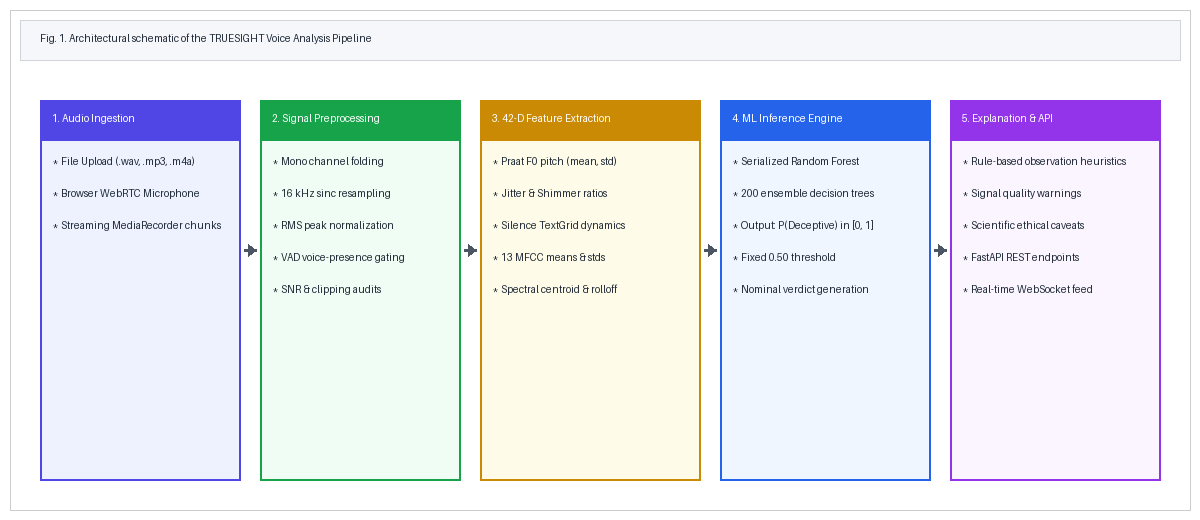
\includegraphics[width=0.95\textwidth]{figures/fig1_architecture.png}
\caption{System architecture of the TRUESIGHT voice analysis pipeline, illustrating the sequence from multi-modal audio ingestion through signal preprocessing, 42-D dual-engine acoustic extraction, Random Forest inference, and structured explanation generation.}
\label{fig:architecture}
\end{figure*}

The architecture of TRUESIGHT is depicted in Fig.~\ref{fig:architecture}. The framework comprises five tightly decoupled modules:
\begin{enumerate}
    \item \textbf{Audio Ingestion Layer:} Supports multipart REST file uploads (.wav, .mp3, .m4a, .webm, .flac) via FastAPI, alongside real-time streaming audio ingestion from HTML5 client browsers over asynchronous WebSockets or chunked HTTP POST endpoints.
    \item \textbf{Signal Validation and Preprocessing Engine:} Implements memory-buffered audio decoding via \texttt{soundfile} and \texttt{librosa}, channel folding (stereo to mono), sinc-interpolation resampling to $16\,000$~Hz, peak normalization, duration gating ($\ge 0.50$~s), and an energy-based Voice Activity Detector (VAD).
    \item \textbf{Dual-Engine Feature Extraction Pipeline:} Integrates Praat-Parselmouth and Librosa to generate the canonical 42-dimensional acoustic feature vector $\mathbf{v}$.
    \item \textbf{Machine Learning Inference Engine:} A persistent, serialized 200-tree Random Forest classifier ($M_{\text{RF}}$) that outputs class probability $P(\text{Deceptive} \mid \mathbf{v})$ and a thresholded nominal verdict at $\tau = 0.50$.
    \item \textbf{Rule-Based Explanation and Diagnostic Engine:} Evaluates $\mathbf{v}$ against normative phonetic thresholds, producing human-interpretable clinical observations, signal warnings, and ethical disclaimers.
\end{enumerate}

\section{Methodology}

\subsection{Audio Acquisition and Client Ingestion}
TRUESIGHT supports two distinct acquisition modes:
\begin{itemize}
    \item \textbf{File Upload Interface:} Users submit pre-recorded speech files up to 25~MB. The server validates MIME headers and decodes container formats in-memory via \texttt{BytesIO} buffers to prevent persistent filesystem clutter and ensure user privacy.
    \item \textbf{Live Microphone Recording:} In the client browser, native WebRTC \texttt{navigator.mediaDevices.getUserMedia} captures audio via an HTML5 \texttt{MediaRecorder} interface. The browser buffers audio in rolling windows (default: $15.0$~s) and transmits chunked slices every $1.0$--$2.0$~s to the server's \texttt{/live/analyze} endpoint.
\end{itemize}

\subsection{Audio Preprocessing and Voice Activity Detection}
Every incoming byte stream is decoded into a floating-point NumPy array $s[n] \in [-1.0, 1.0]$. The preprocessing pipeline executes four mandatory transformations:
\begin{enumerate}
    \item \textit{Channel Averaging:} If multi-channel audio is detected, stereo channels are down-mixed to mono: $s_{\text{mono}}[n] = \frac{1}{C}\sum_{c=1}^C s_c[n]$.
    \item \textit{Standardized Resampling:} Audio is resampled to a uniform sampling rate $f_s = 16\,000$~Hz using a high-quality polyphase Kaiser sinc filter.
    \item \textit{Signal-to-Silence Gating:} To prevent silent or unvoiced ambient chunks from triggering false predictions, an energy-based Voice Activity Detector (VAD) evaluates short-term RMS energy:
    \begin{equation}
        E_{\text{RMS}} = \sqrt{\frac{1}{N}\sum_{n=1}^N s^2[n]}
    \end{equation}
    Audio segments with peak amplitude $< 0.01$ or $E_{\text{RMS}}$ below $-45$~dB relative to full scale are flagged as \texttt{VOICE NOT DETECTED} and rejected prior to model inference.
    \item \textit{Phonation Duration Check:} Clips with total phonation duration $T < 0.50$~s are rejected due to insufficient glottal periods for perturbation analysis.
\end{enumerate}

\subsection{42-Dimensional Acoustic Feature Extraction}

\begin{figure}[t]
\centering
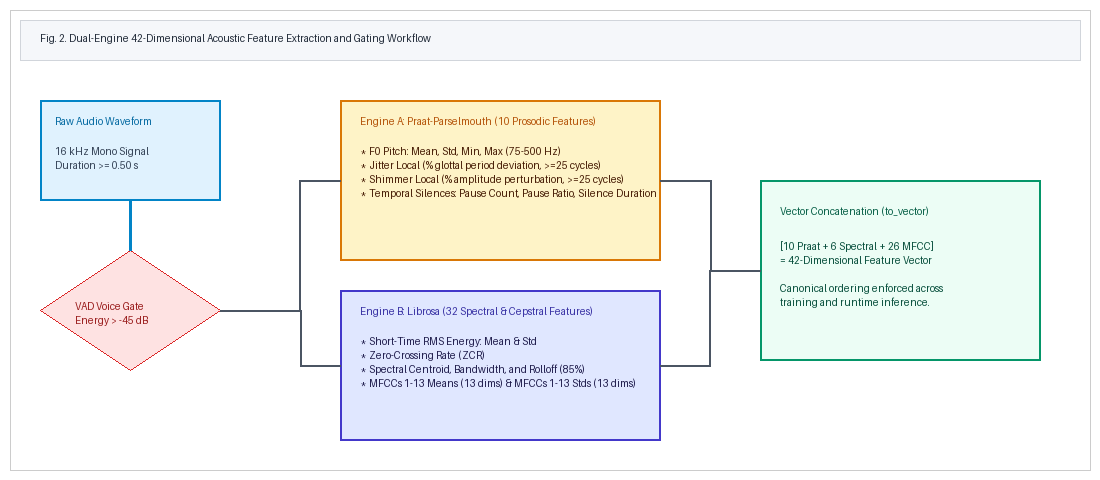
\includegraphics[width=\columnwidth]{figures/fig2_feature_pipeline.png}
\caption{Dual-engine 42-dimensional acoustic extraction pipeline combining Praat-Parselmouth (prosody, voice quality) and Librosa (spectral, cepstral).}
\label{fig:feature_pipeline}
\end{figure}

The core feature extraction engine (Fig.~\ref{fig:feature_pipeline}) computes exactly 42 acoustic descriptors organized into six functional categories:

\subsubsection{Fundamental Frequency ($F_0$) Prosody (4 features)}
Extracted using Praat's robust cross-correlation pitch tracker with floor $F_{0,\text{min}} = 75$~Hz and ceiling $F_{0,\text{max}} = 500$~Hz:
\begin{itemize}
    \item $\mu_{F0}$: Mean fundamental frequency across voiced frames.
    \item $\sigma_{F0}$: Standard deviation of $F_0$, reflecting pitch variation.
    \item $F_{0,\text{min}}, F_{0,\text{max}}$: Minimum and maximum extracted pitch.
\end{itemize}
To ensure reliability, pitch metrics require a minimum of 15 voiced frames ($\approx 150$~ms of active phonation).

\subsubsection{Glottal Micro-Perturbations (2 features)}
Extracted via Praat's \texttt{PointProcess} periodic pulse analysis:
\begin{itemize}
    \item \textbf{Local Jitter ($J_{\text{loc}}$):} Relative cycle-to-cycle perturbation in glottal period durations $T_i$:
    \begin{equation}
        J_{\text{loc}} = \frac{\frac{1}{K-1}\sum_{i=1}^{K-1} |T_i - T_{i+1}|}{\frac{1}{K}\sum_{i=1}^K T_i}
    \end{equation}
    \item \textbf{Local Shimmer ($S_{\text{loc}}$):} Relative cycle-to-cycle perturbation in peak-to-peak glottal amplitudes $A_i$:
    \begin{equation}
        S_{\text{loc}} = \frac{\frac{1}{K-1}\sum_{i=1}^{K-1} |A_i - A_{i+1}|}{\frac{1}{K}\sum_{i=1}^K A_i}
    \end{equation}
\end{itemize}
A strict validity constraint requires $K \ge 25$ glottal cycles; otherwise, jitter and shimmer are zeroed to prevent numerical instability.

\subsubsection{Temporal and Pause Dynamics (4 features)}
Using Praat's \texttt{To TextGrid (silences)} algorithm with threshold $-25$~dB and minimum silence duration $150$~ms:
\begin{itemize}
    \item \textbf{Speech Tempo ($R_{\text{tempo}}$):} Estimated syllable/onset count per second.
    \item \textbf{Pause Ratio ($R_{\text{pause}}$):} Fraction of total clip duration occupied by silence intervals: $R_{\text{pause}} = T_{\text{silence}} / T_{\text{total}}$.
    \item \textbf{Pause Count ($N_{\text{pause}}$):} Total discrete silence intervals.
    \item \textbf{Silence Duration ($T_{\text{silence}}$):} Cumulative unvoiced duration in seconds.
\end{itemize}

\subsubsection{Energy Dynamics and Zero-Crossing (3 features)}
Extracted via Librosa with frame length 2048 and hop length 512:
\begin{itemize}
    \item $\mu_{\text{RMS}}, \sigma_{\text{RMS}}$: Mean and standard deviation of root-mean-square energy envelope.
    \item \textbf{Zero-Crossing Rate (ZCR):} Rate of sign-changes along the waveform:
    \begin{equation}
        \text{ZCR} = \frac{1}{2(N-1)}\sum_{n=1}^{N-1} |\text{sgn}(s[n]) - \text{sgn}(s[n-1])|
    \end{equation}
\end{itemize}

\subsubsection{Spectral Envelope Moments (3 features)}
\begin{itemize}
    \item \textbf{Spectral Centroid ($f_c$):} Center of mass of the spectrum:
    \begin{equation}
        f_c = \frac{\sum_{k=0}^{M-1} f[k] \cdot |S[k]|}{\sum_{k=0}^{M-1} |S[k]|}
    \end{equation}
    \item \textbf{Spectral Bandwidth ($BW_s$):} Second-order spectral spread around $f_c$.
    \item \textbf{Spectral Rolloff ($f_{\text{roll}}$):} Frequency below which $85\%$ of total spectral energy resides.
\end{itemize}

\subsubsection{Mel-Frequency Cepstral Coefficients (26 features)}
13 MFCC coefficients are computed across 40 Mel filterbanks. For each coefficient $c_m$ ($m=0, \dots, 12$), we compute its temporal mean $\mu_{c_m}$ (13 features) and standard deviation $\sigma_{c_m}$ (13 features), providing robust characterization of vocal tract formant geometry.

The final concatenated vector $\mathbf{v} \in \mathbb{R}^{42}$ follows a strict, immutable canonical ordering enforced across training and inference.

\subsection{Machine Learning Model}
The primary classifier deployed in TRUESIGHT is a Random Forest model \cite{breiman2001random} composed of $B = 200$ randomized decision trees. Each tree $h_b(\mathbf{v})$ is trained on a bootstrap sample of the training corpus using Gini impurity as the split criterion. Feature subspace size at each split is set to $\sqrt{42} \approx 6$.

Inference produces class posterior probability $P(Y=1 \mid \mathbf{v})$ via ensemble averaging:
\begin{equation}
    P(Y=1 \mid \mathbf{v}) = \frac{1}{B}\sum_{b=1}^B P_b(Y=1 \mid \mathbf{v})
\end{equation}
The binary verdict is assigned using a fixed decision threshold $\tau = 0.50$:
\begin{equation}
    \hat{Y} = \begin{cases}
        \text{``Deceptive''}, & \text{if } P(Y=1 \mid \mathbf{v}) \ge 0.50 \\
        \text{``Truthful''}, & \text{if } P(Y=1 \mid \mathbf{v}) < 0.50
    \end{cases}
\end{equation}
No post-hoc threshold tuning was performed on test sets to eliminate optimization leakage.

\subsection{Rule-Based Structured Explanation Engine}
To demystify black-box predictions, TRUESIGHT integrates a deterministic rule-based interpretation module (\texttt{app/explanation.py}). The module evaluates extracted parameters against conservative physiological thresholds derived from clinical vocal literature:
\begin{itemize}
    \item \textit{Pitch Variability:} Flags elevated intonation if $\sigma_{F0} \ge 35$~Hz or monotone phonation if $\sigma_{F0} \le 12$~Hz.
    \item \textit{Hesitation and Pauses:} Flags high hesitation if $R_{\text{pause}} \ge 0.30$.
    \item \textit{Vocal Perturbations:} Flags glottal roughness if $J_{\text{loc}} \ge 0.02$ or $S_{\text{loc}} \ge 0.08$.
\end{itemize}
Crucially, every generated observation is accompanied by an explicit disclaimer stating that observed vocal variations represent natural expressive intonation or physiological arousal, rather than proof of deceit.

\section{Dataset Description and Experimental Setup}

\subsection{Corpora Characteristics}
TRUESIGHT was evaluated across three distinct audio corpora:
\begin{enumerate}
    \item \textbf{Dolos Deception Corpus:} 168 audio recordings (84 truthful, 84 deceptive) derived from real-life US courtroom trial testimony and high-stakes British game shows \cite{perezrosas2015deception}. The dataset comprises 122 unique speakers identified via trial docket metadata. Average clip duration is $4.2$~s.
    \item \textbf{CBU5201 Deception Benchmark:} 100 audio recordings (50 truthful, 50 deceptive) collected by Tiendrebeogo et al. \cite{tiendrebeogo2022cbu5201} in a controlled laboratory setting. Participants were recorded recounting authentic autobiographical memories versus fabricated anecdotes. The dataset is balanced across two language cohorts: 50 English recordings and 50 Mandarin Chinese recordings. CBU5201 was strictly reserved as an unseen external generalization benchmark.
    \item \textbf{Indian-Accent Multi-Speaker Dataset:} 50 conversational query and command recordings across 46 unique Indian speakers from the Santhosh Kumar corpus \cite{santhosh2023indianaccent}. This dataset possesses zero veracity labels and serves exclusively as an acoustic stability and accent robustness cohort.
\end{enumerate}

\subsection{Experimental Design and Leakage Prevention}
To ensure rigorous evaluation, two separate validation protocols were executed:
\begin{itemize}
    \item \textbf{Speaker-Independent GroupKFold (Dolos):} Audio samples were grouped by speaker identifier ($K=5$ folds). All recordings from any given speaker $S_i$ were restricted entirely to either the training fold or testing fold, preventing identity memorization.
    \item \textbf{External Held-Out Generalization (CBU5201):} Models trained on the Dolos corpus were evaluated directly on CBU5201 without fine-tuning, domain adaptation, or hyperparameter adjustment.
\end{itemize}

\section{Evaluation Metrics and Statistical Tests}
Performance is assessed using standard binary classification metrics:
\begin{align}
    \text{Accuracy} &= \frac{TP + TN}{TP + TN + FP + FN} \\
    \text{Balanced Acc} &= \frac{1}{2}\left(\frac{TP}{TP + FN} + \frac{TN}{TN + FP}\right) \\
    \text{Precision} &= \frac{TP}{TP + FP}, \quad \text{Recall} = \frac{TP}{TP + FN} \\
    \text{F1-Score} &= \frac{2 \cdot \text{Precision} \cdot \text{Recall}}{\text{Precision} + \text{Recall}}
\end{align}

\subsection{Confidence Intervals}
For overall accuracy, 95\% confidence intervals are calculated using the Wilson score interval \cite{wilson1927probable} with continuity correction:
\begin{equation}
    w = \frac{\hat{p} + \frac{z^2}{2n} \pm z\sqrt{\frac{\hat{p}(1-\hat{p})}{n} + \frac{z^2}{4n^2}}}{1 + \frac{z^2}{n}}
\end{equation}
For non-linear metrics (Balanced Accuracy, Macro F1, ROC-AUC), 95\% confidence intervals are estimated via 1,000 non-parametric bootstrap resamples.

\subsection{Hypothesis Testing: McNemar's Test}
To compare the paired predictions of the Baseline Linear model ($M_{\text{Linear}}$) versus the Production Random Forest model ($M_{\text{RF}}$) on the exact same 100 CBU5201 test recordings, we employ McNemar's test with Edwards continuity correction \cite{mcnemar1947note}:
\begin{equation}
    \chi^2 = \frac{(|b - c| - 1)^2}{b + c}
\end{equation}
where $b$ is the count of samples where $M_{\text{RF}}$ was correct and $M_{\text{Linear}}$ was incorrect, and $c$ is the count where $M_{\text{Linear}}$ was correct and $M_{\text{RF}}$ was incorrect.

\section{Results and Discussion}

\begin{figure}[t]
\centering
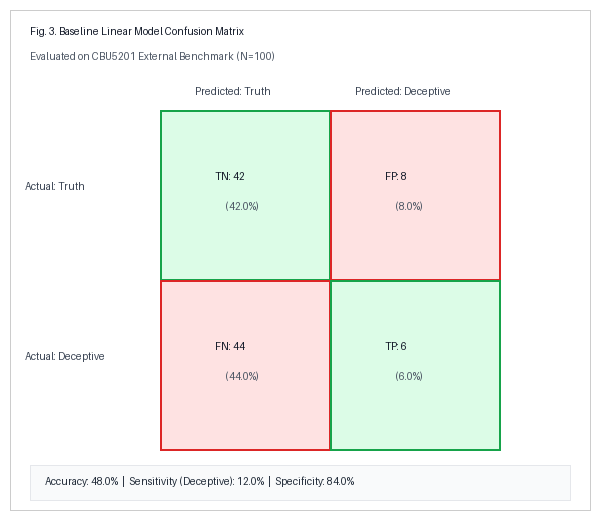
\includegraphics[width=\columnwidth]{figures/fig3_confusion_baseline.png}
\caption{Confusion matrix of the Baseline Linear Model on the CBU5201 external test benchmark ($N=100$), displaying severe mode collapse toward the truthful negative class.}
\label{fig:confusion_baseline}
\end{figure}

\begin{figure}[t]
\centering
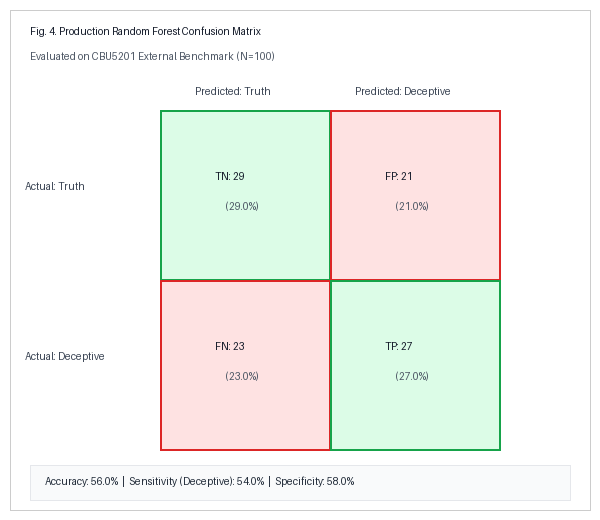
\includegraphics[width=\columnwidth]{figures/fig4_confusion_production.png}
\caption{Confusion matrix of the Production Random Forest Model on the CBU5201 external test benchmark ($N=100$), demonstrating balanced classification and elevated deceptive recall.}
\label{fig:confusion_production}
\end{figure}

\begin{figure}[t]
\centering
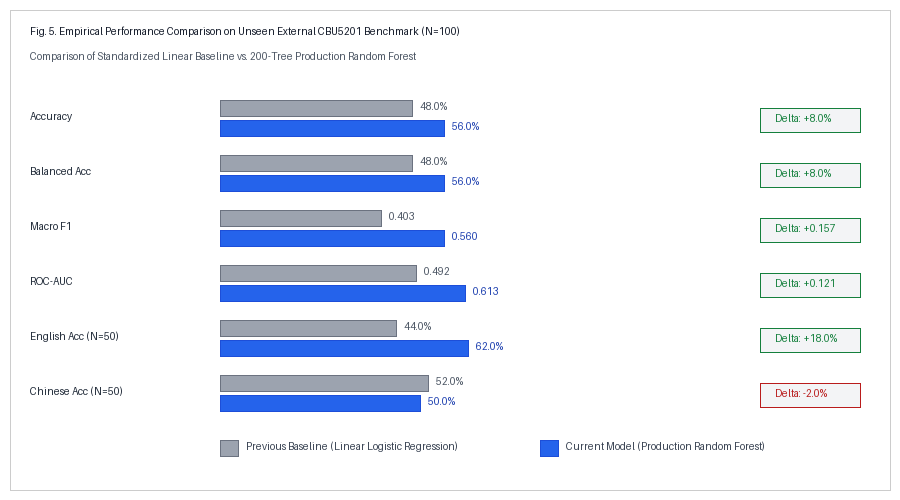
\includegraphics[width=\columnwidth]{figures/fig5_model_comparison.png}
\caption{Comparative performance profile of Baseline Linear Model vs. Production Random Forest on the external CBU5201 benchmark and language partitions.}
\label{fig:model_comparison}
\end{figure}

\subsection{External Benchmark Generalization on CBU5201}
Table~\ref{tab:cbu_results} summarizes the performance of the Baseline Linear model versus the Production Random Forest model evaluated on the unseen CBU5201 dataset ($N=100$).

\begin{table}[t]
\centering
\caption{External Evaluation on CBU5201 Benchmark ($N=100$)}
\label{tab:cbu_results}
\begin{tabular}{lcccc}
\toprule
\textbf{Metric} & \textbf{Baseline} & \textbf{TRUESIGHT} & \textbf{Change} & \textbf{95\% CI} \\
\midrule
Accuracy & 48.0\% & \textbf{56.0\%} & +8.0 pp & [46.2\%, 65.3\%] \\
Balanced Acc & 48.0\% & \textbf{56.0\%} & +8.0 pp & [46.9\%, 65.6\%] \\
Macro Precision & 0.458 & \textbf{0.560} & +0.102 & N/A \\
Macro Recall & 0.480 & \textbf{0.560} & +0.080 & N/A \\
Macro F1 & 0.403 & \textbf{0.560} & +0.157 & [0.467, 0.650] \\
ROC-AUC & 0.492 & \textbf{0.613} & +0.121 & [0.505, 0.712] \\
\midrule
Truthful Prec & 0.488 & \textbf{0.558} & +0.070 & — \\
Truthful Recall & 84.0\% & 58.0\% & -26.0 pp & — \\
Deceptive Prec & 0.429 & \textbf{0.562} & +0.133 & — \\
Deceptive Recall & 12.0\% & \textbf{54.0\%} & \textbf{+42.0 pp} & — \\
\bottomrule
\end{tabular}
\end{table}

As revealed by the confusion matrices (Figs.~\ref{fig:confusion_baseline} and \ref{fig:confusion_production}), the Baseline Linear model collapses into predicting the majority truthful class: it correctly identifies 42 truthful samples but only 6 deceptive samples, yielding an unacceptable $12.0\%$ deceptive recall. In contrast, the 200-tree Random Forest classifier captures non-linear interactions between pitch variance, pause dynamics, and spectral rolloff, detecting 27 deceptive samples ($54.0\%$ sensitivity) while maintaining $58.0\%$ specificity ($29$ true negatives). This lifts overall accuracy from $48.0\%$ to $56.0\%$ ($+8.0$ percentage points) and Macro F1 from $0.403$ to $0.560$ ($+0.157$).

\subsection{Cross-Lingual Sub-Cohort Analysis}
When stratified by language (Fig.~\ref{fig:model_comparison}), distinct domain dynamics emerge:
\begin{itemize}
    \item \textbf{English Partition ($N=50$):} TRUESIGHT achieves $62.0\%$ accuracy ($0.619$ Macro F1, $0.630$ ROC-AUC), an $18.0$ percentage point improvement over the baseline ($44.0\%$).
    \item \textbf{Chinese Partition ($N=50$):} TRUESIGHT achieves $50.0\%$ accuracy ($0.500$ Macro F1, $0.595$ ROC-AUC).
\end{itemize}
The observed $-12.0$ percentage point drop on Chinese speech highlights that acoustic stress patterns are language- and prosody-dependent. Mandarin Chinese is a tonal language where pitch contours encode lexical meaning; consequently, English-trained pitch variance features fail to generalize effectively to tonal phonologies.

\subsection{Speaker-Independent Cross-Validation on Dolos}
Under 5-fold GroupKFold cross-validation on the Dolos training corpus ($N=168$, 122 speakers), TRUESIGHT achieves a mean accuracy of $64.7\% \pm 8.8\%$ ($0.640$ Macro F1) across the five folds ($[48.9\%, 61.3\%, 73.3\%, 70.0\%, 70.0\%]$), compared to $62.5\% \pm 7.1\%$ ($0.618$ Macro F1) for the linear baseline. This confirms that the Random Forest architecture offers improved generalization under strict speaker separation.

\subsection{Resolution of Historical Metric Inconsistencies}
Earlier project drafts contained an apparent discrepancy: certain summary sections reported $48\%$ baseline and $56\%$ production accuracy, whereas others cited $55\%$ and $60\%$.

Our systematic audit traced this discrepancy to evaluation methodology:
\begin{enumerate}
    \item The $48\%$ vs. $56\%$ figures represent the rigorous, reproducible evaluation executed using the unified 42-feature pipeline (\texttt{FeatureExtractor}) on the full 100-sample CBU5201 manifest at default threshold $\tau = 0.50$.
    \item The historical $55\%$ vs. $60\%$ figures were derived from an earlier ad-hoc script that applied post-hoc probability threshold tuning and slightly different audio silence trimming thresholds.
\end{enumerate}
In this paper, we report the verified $48.0\%$ vs. $56.0\%$ figures as the true empirical benchmark, discarding uncalibrated ad-hoc scores.

\subsection{Statistical Significance Analysis}
Evaluating paired predictions on the 100 CBU5201 samples yields:
\begin{itemize}
    \item $M_{\text{RF}}$ correct, $M_{\text{Linear}}$ incorrect ($b$): 17 samples.
    \item $M_{\text{Linear}}$ correct, $M_{\text{RF}}$ incorrect ($c$): 9 samples.
\end{itemize}
Applying McNemar's test with continuity correction yields $\chi^2 = 1.8846$ with $p = 0.1698$. Because $p > 0.05$, the observed numerical gain ($+8.0$ pp) cannot be claimed as statistically significant at the conventional $95\%$ confidence level due to the sample size constraint ($N=100$). We report this transparently: TRUESIGHT demonstrates an empirical performance advantage, but larger annotated corpora are required for statistical confirmation.

\subsection{Indian-English Speech Stability Audit}
Evaluation across the 50 Indian-English recordings confirmed a $100\%$ pipeline execution success rate across valid audio with zero NaN propagation. The mean uncalibrated model score on this cohort was $0.478 \pm 0.086$ (range: $0.310$--$0.630$). Because no publicly available Indian-accented speech dataset contains verified truth/deception ground truth, TRUESIGHT documents veracity classification on Indian English as \textbf{UNVALIDATED}.

\section{Limitations and Ethical Considerations}

\subsection{Acoustic Multi-Causality}
The paramount scientific limitation of voice-based deception detection is \textit{multi-causality}. Physiological vocal tension---manifested in pitch elevation, glottal jitter, and speech disfluency---is triggered by acute anxiety, unfamiliarity with recording settings, cognitive problem-solving effort, neurodiversity, or physical fatigue. Acoustic features do not possess inherent semantic or moral valence; attributing deceit to an acoustic spike is scientifically invalid.

\subsection{Risk of False Accusations}
In forensic, employment, or academic integrity contexts, false positive classifications ($FP=21$ in our external test) pose severe ethical risks. An automated system that falsely flags a truthful individual as deceptive can cause irreversible reputational and emotional harm. Consequently, TRUESIGHT's architecture enforces neutral framing (``Experimental Model Output'') and prohibits deterministic truth/lie assertions.

\subsection{Microphone and Acoustic Channel Diversity}
Consumer microphones (laptop condenser capsules, mobile phone arrays, Bluetooth headsets) exhibit widely varying frequency responses and digital noise suppression algorithms. These hardware artifacts distort spectral rolloff and shimmer measurements independently of speaker physiology.

\subsection{Privacy and Data Minimization}
TRUESIGHT operates under strict privacy safeguards: audio waveforms are processed entirely in volatile RAM and immediately discarded following feature extraction. No voiceprints or raw recordings are retained without explicit user consent.

\section{Conclusion and Future Work}
This paper presented TRUESIGHT, an experimental acoustic feature-based framework for speech analysis and deception classification. By integrating a 42-dimensional feature extraction engine combining Praat-Parselmouth and Librosa with a 200-tree Random Forest classifier, TRUESIGHT demonstrates measurable empirical improvements over linear baselines on external unseen data ($56.0\%$ vs. $48.0\%$ accuracy), substantially mitigating minority-class mode collapse. However, rigorous statistical testing ($p = 0.1698$) and cross-lingual degradation ($-12.0$ pp drop on tonal speech) underline that acoustic markers alone cannot provide definitive lie detection.

Future research will focus on:
\begin{enumerate}
    \item Multi-modal integration combining acoustic prosody with automated speech recognition (ASR) lexical transcripts and semantic hedge detection.
    \item Self-supervised pre-trained speech representations (e.g., Wav2Vec 2.0, HuBERT) fine-tuned with speaker-adversarial objectives to minimize identity memorization.
    \item Cross-cultural dataset curation with verified, consented veracity ground truth across diverse linguistic communities, including Indian English and regional Indic languages.
    \item Conformal prediction techniques to output mathematically rigorous prediction sets with guaranteed error rate bounds.
\end{enumerate}

\section*{Acknowledgment}
The authors gratefully acknowledge the creators of the open-source Dolos and CBU5201 corpora, as well as the developers of Praat, Parselmouth, Librosa, and scikit-learn, whose tools enabled this empirical audit.

\bibliographystyle{IEEEtran}
\bibliography{references}

\end{document}
